\subsection{Praktische Anwendung der FM-Synthese}
\FloatBarrier
\subsubsection{Nachbildung eines Instruments}
Da es bei der FM Synthese schwer ist im Vorfeld zu wissen was für ein Spektrum durch die Synthese erzeugt wird, ist es schwer und benötigt einige Experimente um mit dieser Technik ein echt wirkendes Instrument nachzubilden.
Trotzdem gibt es einige Methoden den generierten Klang natürlicher wirken zu lassen. Diese werden im weiteren Verlauf diese Kapitels vorgestellt und anschließend versucht den Klang eines Tones einer Querflöte nachzubilden.

Da bei vielen Instrumenten die Lautstärke während der Laufzeit eines Tones variiert, und ein abruptes Ein oder Ausschalten des Tones nicht realistisch klingt, ist die Nutzung einer ADSR-Hüllkurve ein wichtiger Bestandteil der Nachbildung eines Instrumentes. ADSR steht für die einzelnen Phasen eines Tones: Attack, Decay, Sustain und Release. Diese Phasen sollen hier vereinfacht erklärt werden. Beim Drücken einer Taste wird der Ton angeschlagen und die Lautstärke des Tones steigt schnell bis zu einem maximal Wert an. Diese Phase wird Attack-Phase genannt. Nachdem die maximale Lautstärke erreicht wurde, startet die Decay Phase. In dieser Phase sinkt die Lautstärke schnell auf einen geringeren Wert ab. Danach befindet sich der Ton in der Sustain Phase und die Lautstärke bleibt gleich, solange der Ton gespielt wird. Sobald die Taste losgelassen wird, nimmt die Lautstärke wieder bis zu ihrem minimal Wert ab. In Abbildung \ref{fig:defaultADSR} ist der Verlauf der Lautstärke einer Standard ADSR-Hüllkurve noch einmal grafisch dargestellt.

\begin{figure} [ht]
\centering
  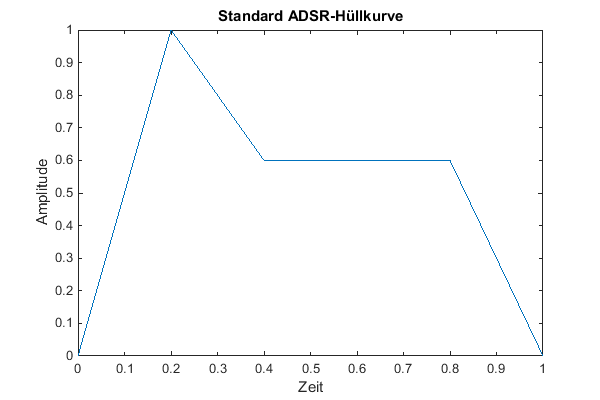
\includegraphics[width=0.5\textwidth]{standardadsr.png}
\caption{Standard ADSR-Hüllkurve}
\label{fig:defaultADSR}
Quelle: Eigene Darstellung mit Matlab
\end{figure}

Da allerdings bei vielen Instrumenten die Lautstärke in den einzelnen Phasen der ADSR-Hüllkurve nicht gleichmäßig steigt oder sinkt, ist es nötig die Kurven beliebig Komplex abbilden zu können. Zum Beispiel steigt bei vielen Instrumenten die Lautstärke in der Attack Phase exponentiell an und fällt in der Decay und Release Phase auch exponentiell ab. Manche Synthesizer bieten zusätzlich auch noch eine Hold Phase vor der Attack Phase, da manche Instrumente einige Zeit benötigen bis sie nach dem Anschlagen des Tones in die Attack Phase eintreten. In Abbildung \ref{fig:blechblasadsr} und \ref{fig:klavieradsr} wurden weitere für Instrumenten typische Hüllkurven dargestellt.

\begin{figure} [ht]
\centering
  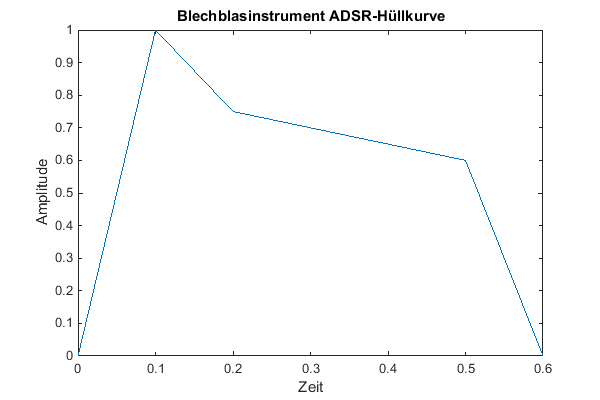
\includegraphics[width=0.5\textwidth]{blechblasadsr.png}
\caption{Typische ADSR-Hüllkurve eines Blechblasinstrumentes}
\label{fig:blechblasadsr}
Quelle: Eigene Darstellung mit Matlab
\end{figure}

\begin{figure} [ht]
\centering
  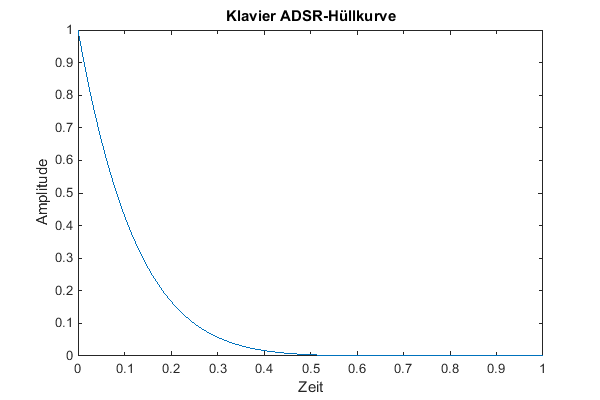
\includegraphics[width=0.5\textwidth]{klavieradsr.png}
\caption{Typische ADSR-Hüllkurve eines Klaviers}
\label{fig:klavieradsr}
Quelle: Eigene Darstellung mit Matlab
\end{figure}

Auch wenn das Hinzufügen einer ADSR-Hüllkurve den Klang des synthetisierten Tones schon stark verbessert, hört sich der erzeugte Ton leider noch nicht wie ein echtes Instrument an. Eine weitere Möglichkeit den Ton weiter zu verbessern, stellt die Varrierung des Modulationsindex über die Zeit oder die Amplitude dar. Somit kann die Anzahl der Seitenfrequenzen verändert werden. Bei Blasinstrumenten wird der Modulationsindex typischerweise über die Amplitude (also mit der ADSR-Hüllkurve) variiert. \cite[S. 532]{chowningPaper}

Abgesehen von der einfachen Frequenz Modulation ist es auch möglich mehrere Modulatoren zu verwenden. Diese können in reihe oder parallel geschaltet werden. Außerdem kann auch die sogenannte Feedback Frequenz Modulation genutzt werden, welche das vorran gegangene Signal moduliert. Feedback FM wird vorallem eingesetzt um rauschen zu erzeugen, es kann aber auch ein sehr komplexes Spektrum mit vielen Seitenfrequenzen erzeugen. Komplexe FM-Synthese findet Einsatz wenn die normale FM-Synthese nicht ausreichend komplexe Spektren erzeugt. Dies kann der Fall sein wenn mehrere stetig fallende Seitenfrequenzen erzeugt werden sollen. Wenn bei einfacher FM-Synthese der Modulationsindex erhöht wird um mehr Seitenfrequenzen zu erzeugen, nimmt die Stärke der Grundfrequenz - definiert durch die Bessel Funktion - immer weiter ab und verteilt sich auf die Seitenfrequenzen \ref{bulli:besselModIndexZusammenahang}. Um dies zu vermeiden können die Modulatoren verschachtelt werden - nachzulesen im Kapitel Komplexe Frequenzmodulation (bla)

Eine reihe an Filtern kann genutzt werden um das von der FM Synthese erzeugte Signal zu verbessern. Diese Filter können mittels additive oder subtraktive Synthese das Signal manipulieren und so ungewollte Frequenzen herausfiltern. Typische Filter sind: Hochpassfilter, Tiefpassfilter, Bandpass und Bandsperre. 



Kein Instrument erzeugt einen hundertprozentigen Klang. Bei Luftverwirblungen und Unebenheiten des Instrumentes wird Rauschen erzeugt. Dieses Rauschen trägt zum typischen Klangbild eines Instrumentes bei und sollte auch nachgebildet werden. Ein Rauschen kann mittels FM Feedback Generator erzeugt werden, dafür muss der Modulationsindex der Feedback FM-Synthese sehr hoch angesetzt werden. Anschließend kann dieses Rauschen mittels Multibandpassfilter um die jeweiligen ausgeprägten Frequenzen gefiltert werden. Würde das Rauschen nicht gefiltert werden, würde man neben dem Ton, das Rauschen als solches wahrnehmen.


Raumhall

Um den Klang des Synthetisierten Tones noch realistischer zu machen, kann er mit einem Raumhall veredelt werden.

Einschwingvorgang

Jedes Instrument hat seine eigene charakteristische Einschwingphase, bei vielen Instrumenten ist es eine kurze Hold Phase, die mittels ADSR-Hüllkurve realisiert werden kann.


Beispiel Querflöte

Im Laufe dieses Kapitels soll ein Ton einer Querflöte mittels FM-Synthese erzeugt und mit den oben beschriebenen Techniken verfeinert werden. Alle Beispiele sind in Matlab erstellt und können mit den beiliegenden Dateien nachgestellt werden. In Abbildung \ref{fig:plotFluteOrig} sind Spektrogram, Waveform und Spektrum des Originalen Querflöten Tones abgebildet. Mit den Information aus den vorliegenden Grafiken wird versucht, diesen spezifischen Ton nachzubilden.

\begin{figure} [ht]
\centering
  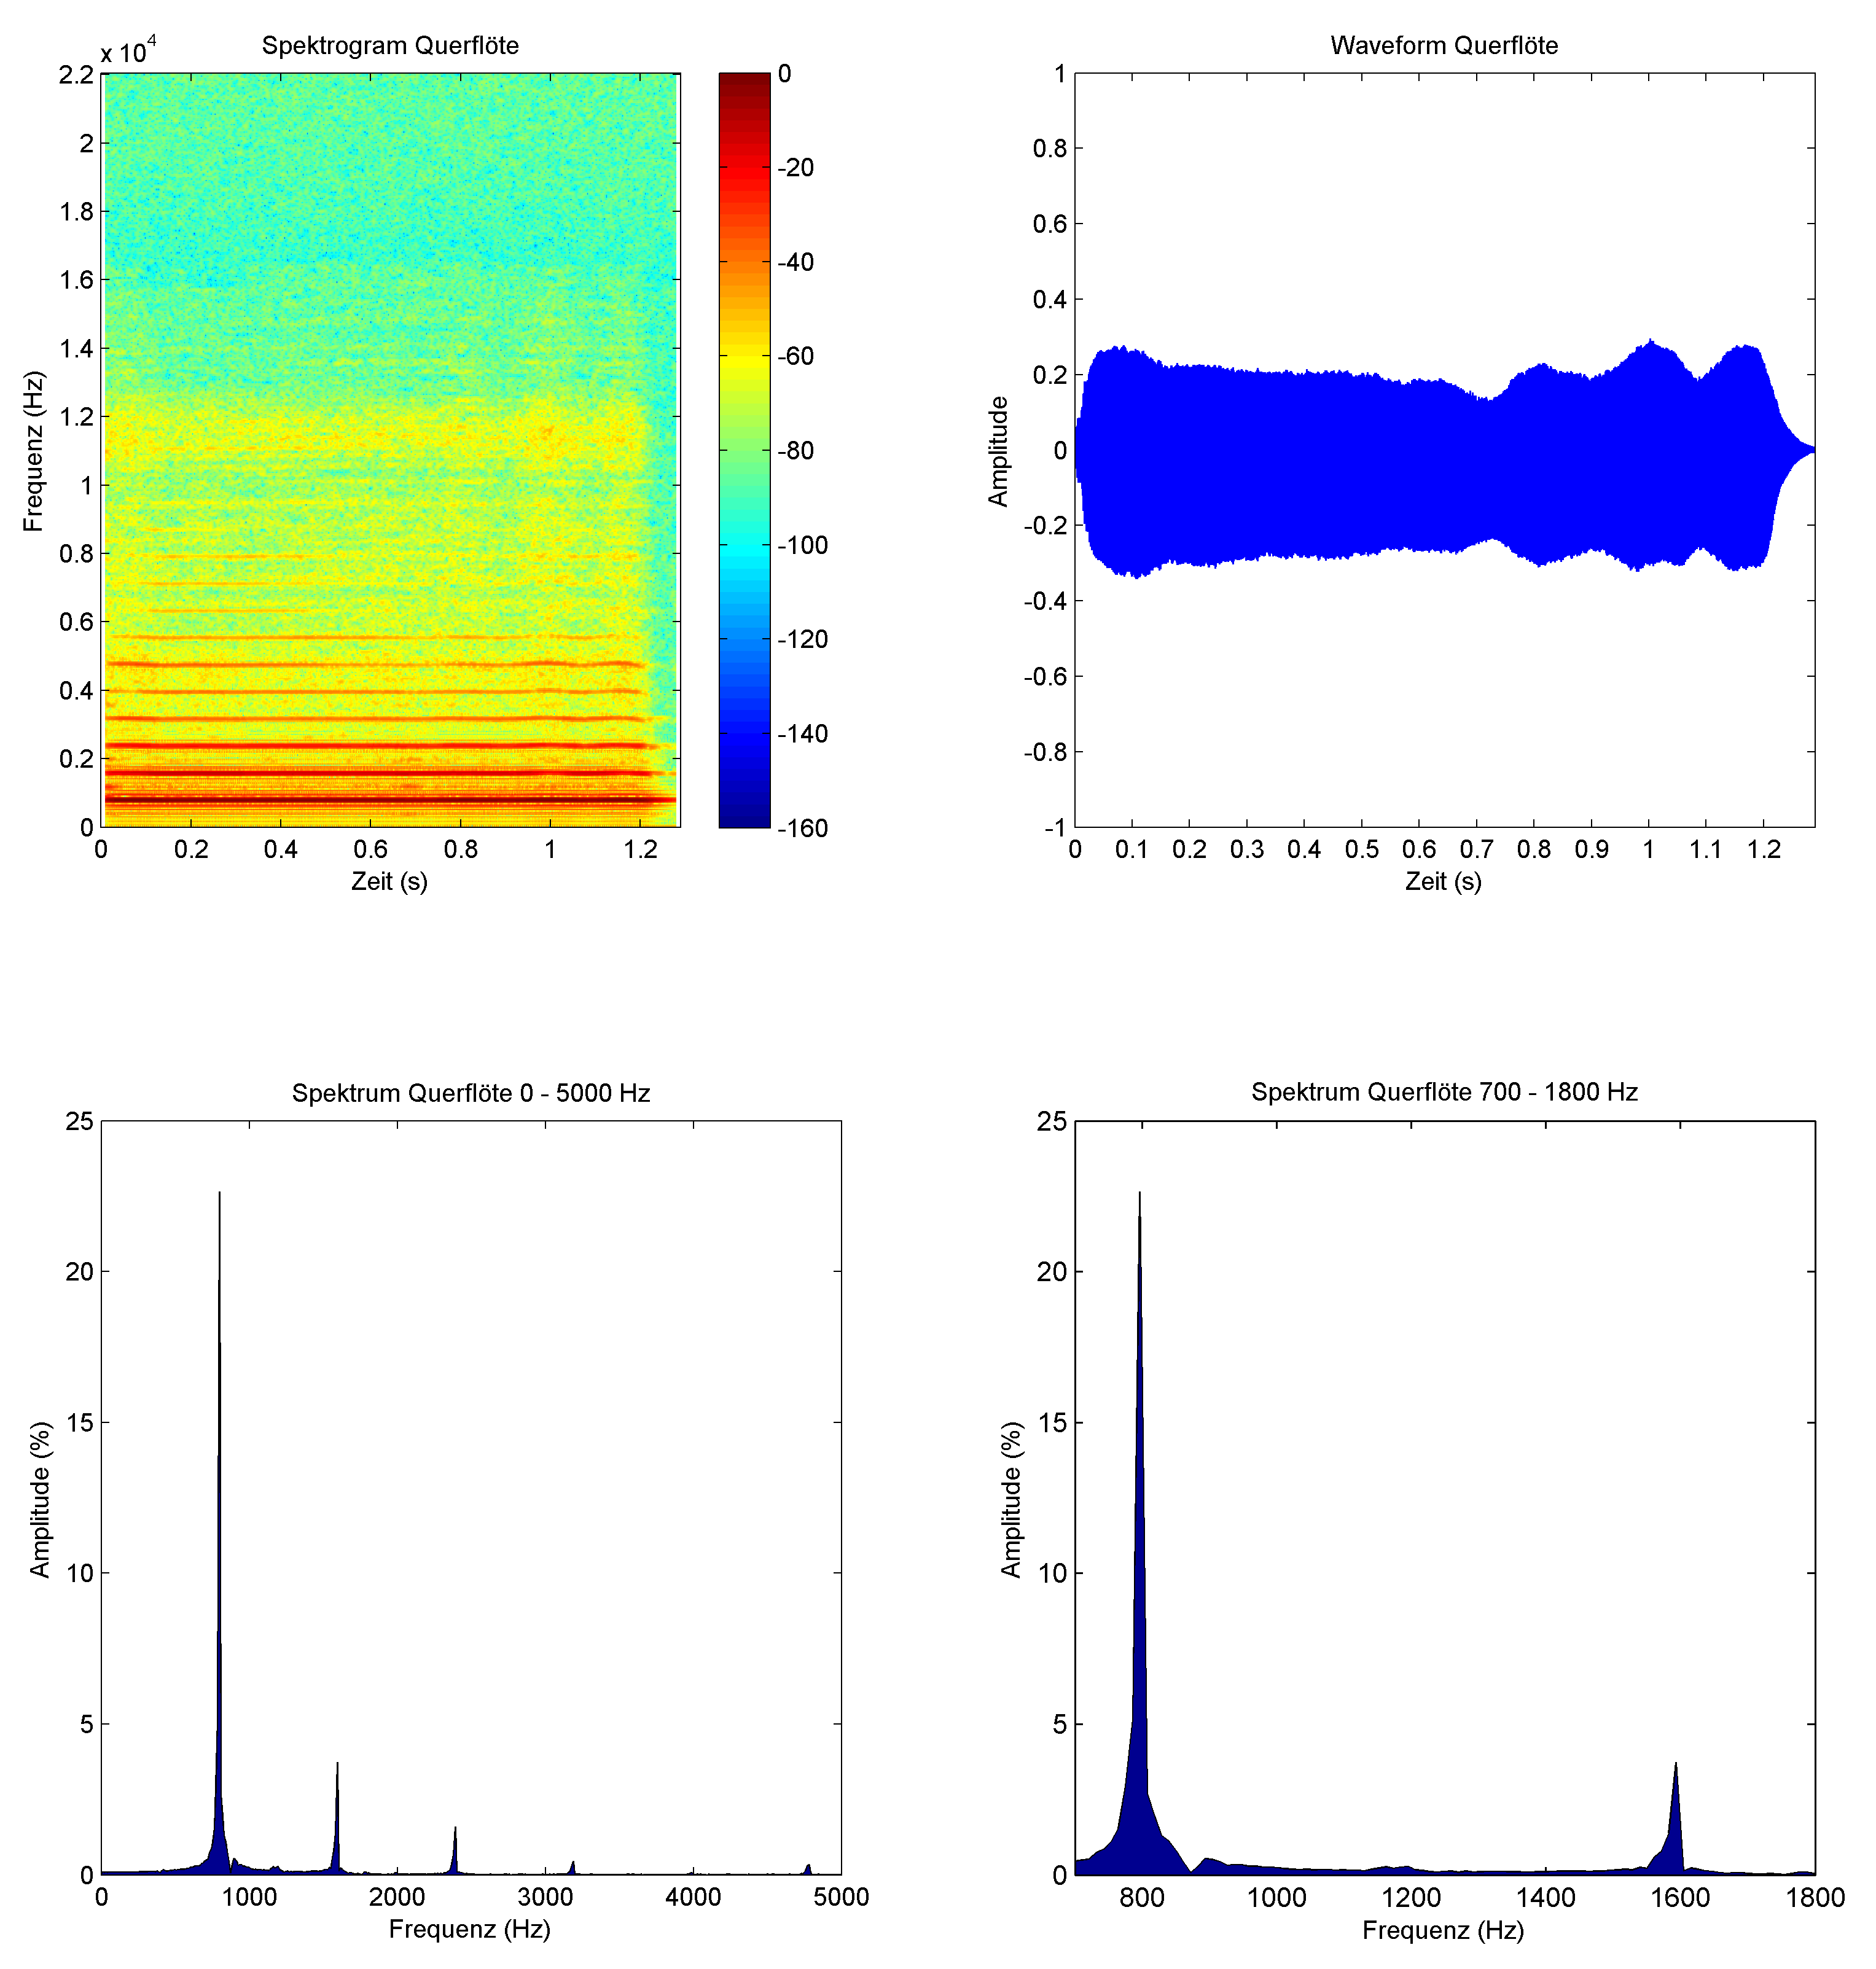
\includegraphics[width=1\textwidth]{plotFluteOrig.png}
\caption{Plot des Spektrograms, der Waveform und des Spektrums eines echten Tones einer Querflöte}
\label{fig:plotFluteOrig}
Quelle: Eigene Darstellung mit Matlab
\end{figure}

Anhand des Spektrums können wir bereits einige Erkenntnisse für unsere FM-Synthese auslesen. Zunächst ist zu erkennen das die am stärksten ausgeprägte Frequenz bei etwa 800 Hz liegt. Bei genauerer Betrachtung wird sichtbar das die Frequenz nicht exakt bei 800 Hz sondern bei 796.75 Hz ihren maximalen Ausschlag erreicht. Dies entspricht am ehesten einem G5 mit 784 Hz \cite[S. 181]{borucki}. Diese Frequenz (796.75 Hz) werden wir bei der FM-Synthese als Träger Frequenz nutzen. Im Spektrum sind außerdem noch mehrere Seitenfrequenzen zu sehen. Die erste dieser Seitenfrequenzen befindet sich bei etwa dem doppelten der Grundfrequenz. Bei genauerer Betrachtung wird sichtbar das sie ihren maximalen Amplitudenwert wirklich genau bei dem doppeltem der Grundfrequenz (1593.5 Hz) hat. Das bedeutet der Abstand zwischen Grundfrequenz und erster Seitenfrequenz ist genauso groß wie der Abstand von 0 Hz bis zur Grundfrequenz, hierbei ist zu bemerken das der Abstand von einem ganzzahligen Multiplikator mit der Grundfrequenz typisch für einen harmonischen Ton ist \cite[S. 528]{chowningPaper}. Die nächsten Seitenfrequenzen haben jeweils wieder den selben Abstand von 796.75 Hz zur jeweiligen vorangegangenen Seitenfrequenz. Aus dieser Beobachtung können wir unsere Modulationsfrequenz von 796.75 Hz schließen. Anhand der Anzahl der sichtbaren Seitenfrequenzen im Spektrum können wir eine ungefähre Abschätzung unseres Modulationsindexes wagen. Da zwischen Modulationsindex und Anzahl der Seitenfrequenzen etwa gilt I+2 = n (bla) wird als Modulationsindex fürs erste einmal 0.5 angenommen. 

\begin{figure} [ht]
\centering
  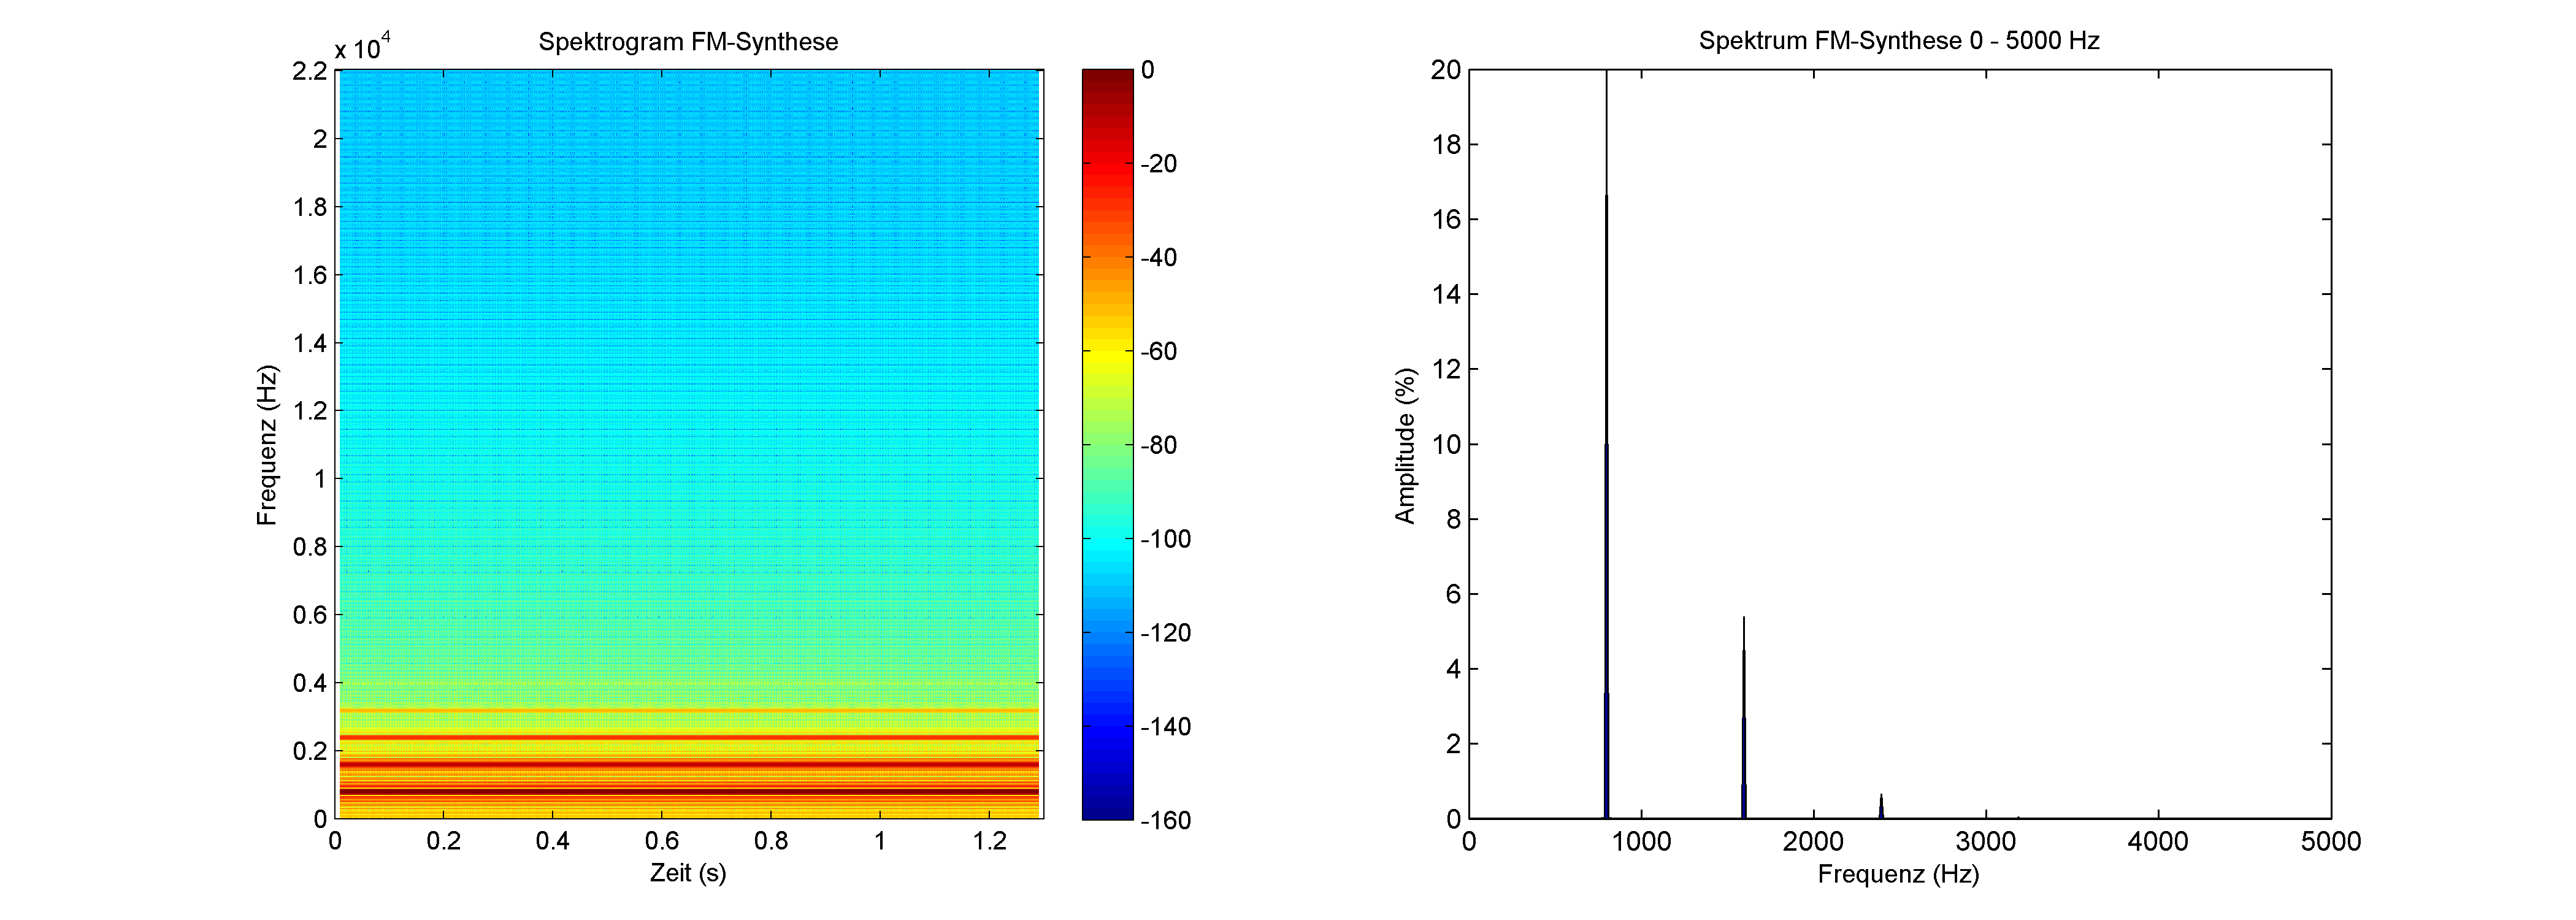
\includegraphics[width=1\textwidth]{plotFMSyntheseI05.png}
\caption{Plot des Spektrograms und des Spektrums der FM-Synthese mit den Parametern fc = 796.75 Hz, fm = fc und I = 0.5 }
\label{fig:plotFMSyntheseI05}
Quelle: Eigene Darstellung mit Matlab
\end{figure}

Ein erstes Spektrum der FM-Synthese mit den eben festgelegten Werten kann in Abbildung \ref{fig:plotFMSyntheseI05} begutachtet werden. Beim evaluieren der Ergebnisse dieses Spektrums fällt auf das die erste Seitenfrequenz im Verhältnis zur Grundfrequenz einen viel Stärkeren Ausschlag aufweist als es bei der Querflöte der Fall ist. Außerdem fällt danach die Amplitude der 2. und 3. Seitenfrequenz viel stärker ab als bei dem Instrument. Sieht man sich jetzt noch das Spektrogram in Abbildung \ref{fig:plotFMSyntheseI05} an, fällt im Vergleich zum Spektrogram der Querflöte auf, das bei der FM-Synthese sehr viel weniger Seitenfrequenzen erzeugt werden. Die Seitenfrequenzen bei 4000 Hz und darüber sind bei dem Instrument noch deutlich sichtbar während sie bei der FM-Synthese schon bei 4000 Hz kaum noch existent sind. Versucht man jetzt den Modulationsindex zu erhöhen um mehr Seitenfrequenzen zu erzeugen verlagert sich die Amplitude unserer Träger Frequenz auf die Seitenfrequenzen, damit werden die Seitenfrequenz stärker und die Träger Frequenz schwächer, zu sehen in Abbildung \ref{fig:spektrumFMSyntheseI4}.

\begin{figure} [ht]
\centering
  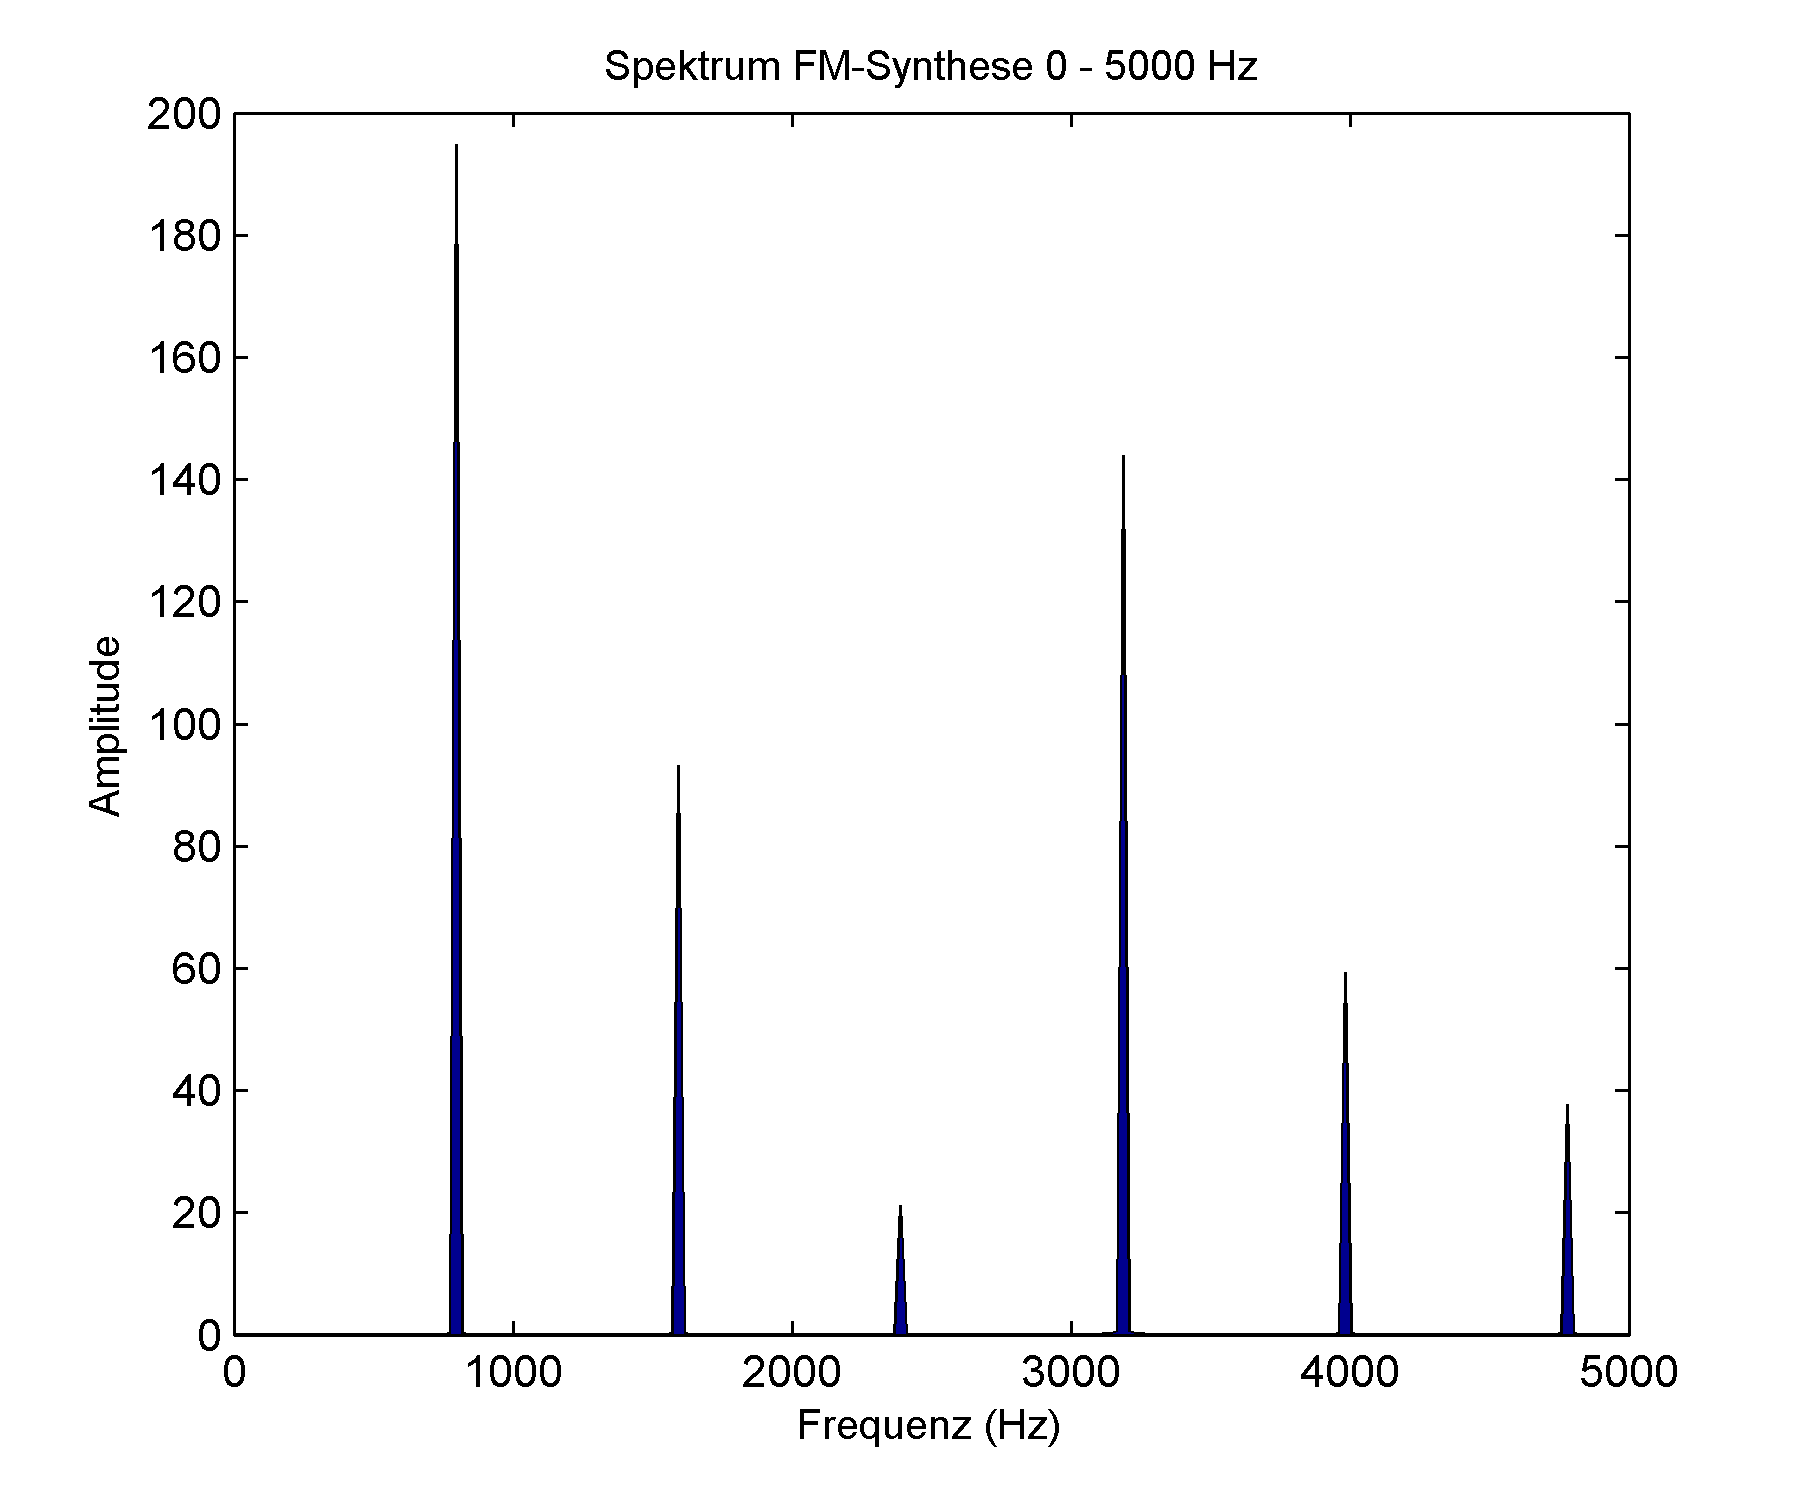
\includegraphics[width=0.5\textwidth]{spektrumFMSyntheseI4.png}
\caption{Plot des Spektrums der FM-Synthese mit den Parametern fc = 796.75 Hz, fm = fc und I = 4}
\label{fig:spektrumFMSyntheseI4}
Quelle: Eigene Darstellung mit Matlab
\end{figure}

Um dieses Verhalten zu umgehen müssen wir uns der Komplexen FM-Synthese widmen. Hier werden mehrere Modulatoren verschachtelt um eine größere Anzahl an Seitenfrequenzen zu erzeugen. Allerdings ist es bei der Komplexen FM-Synthese schwer vorauszusagen wie stark die Amplituden der einzelnen Seitenfrequenzen ausgeprägt sind, deshalb braucht es hier einige Experimente um auf das gewünschte Ergebnis zu stoßen. In Abbildung \ref{fig:plotFMSyntheseKomplex4Mod} sehen sie das Ergebnis der FM-Synthese mit 4 Modulatoren. Dieses Spektrum ähnelt dem der Querflöte schon sehr viel stärker und auch das Spektrogram weißt in den Intensitäten der Seitenfrequenzen eine deutliche Ähnlichkeit auf.

\begin{figure} [ht]
\centering
  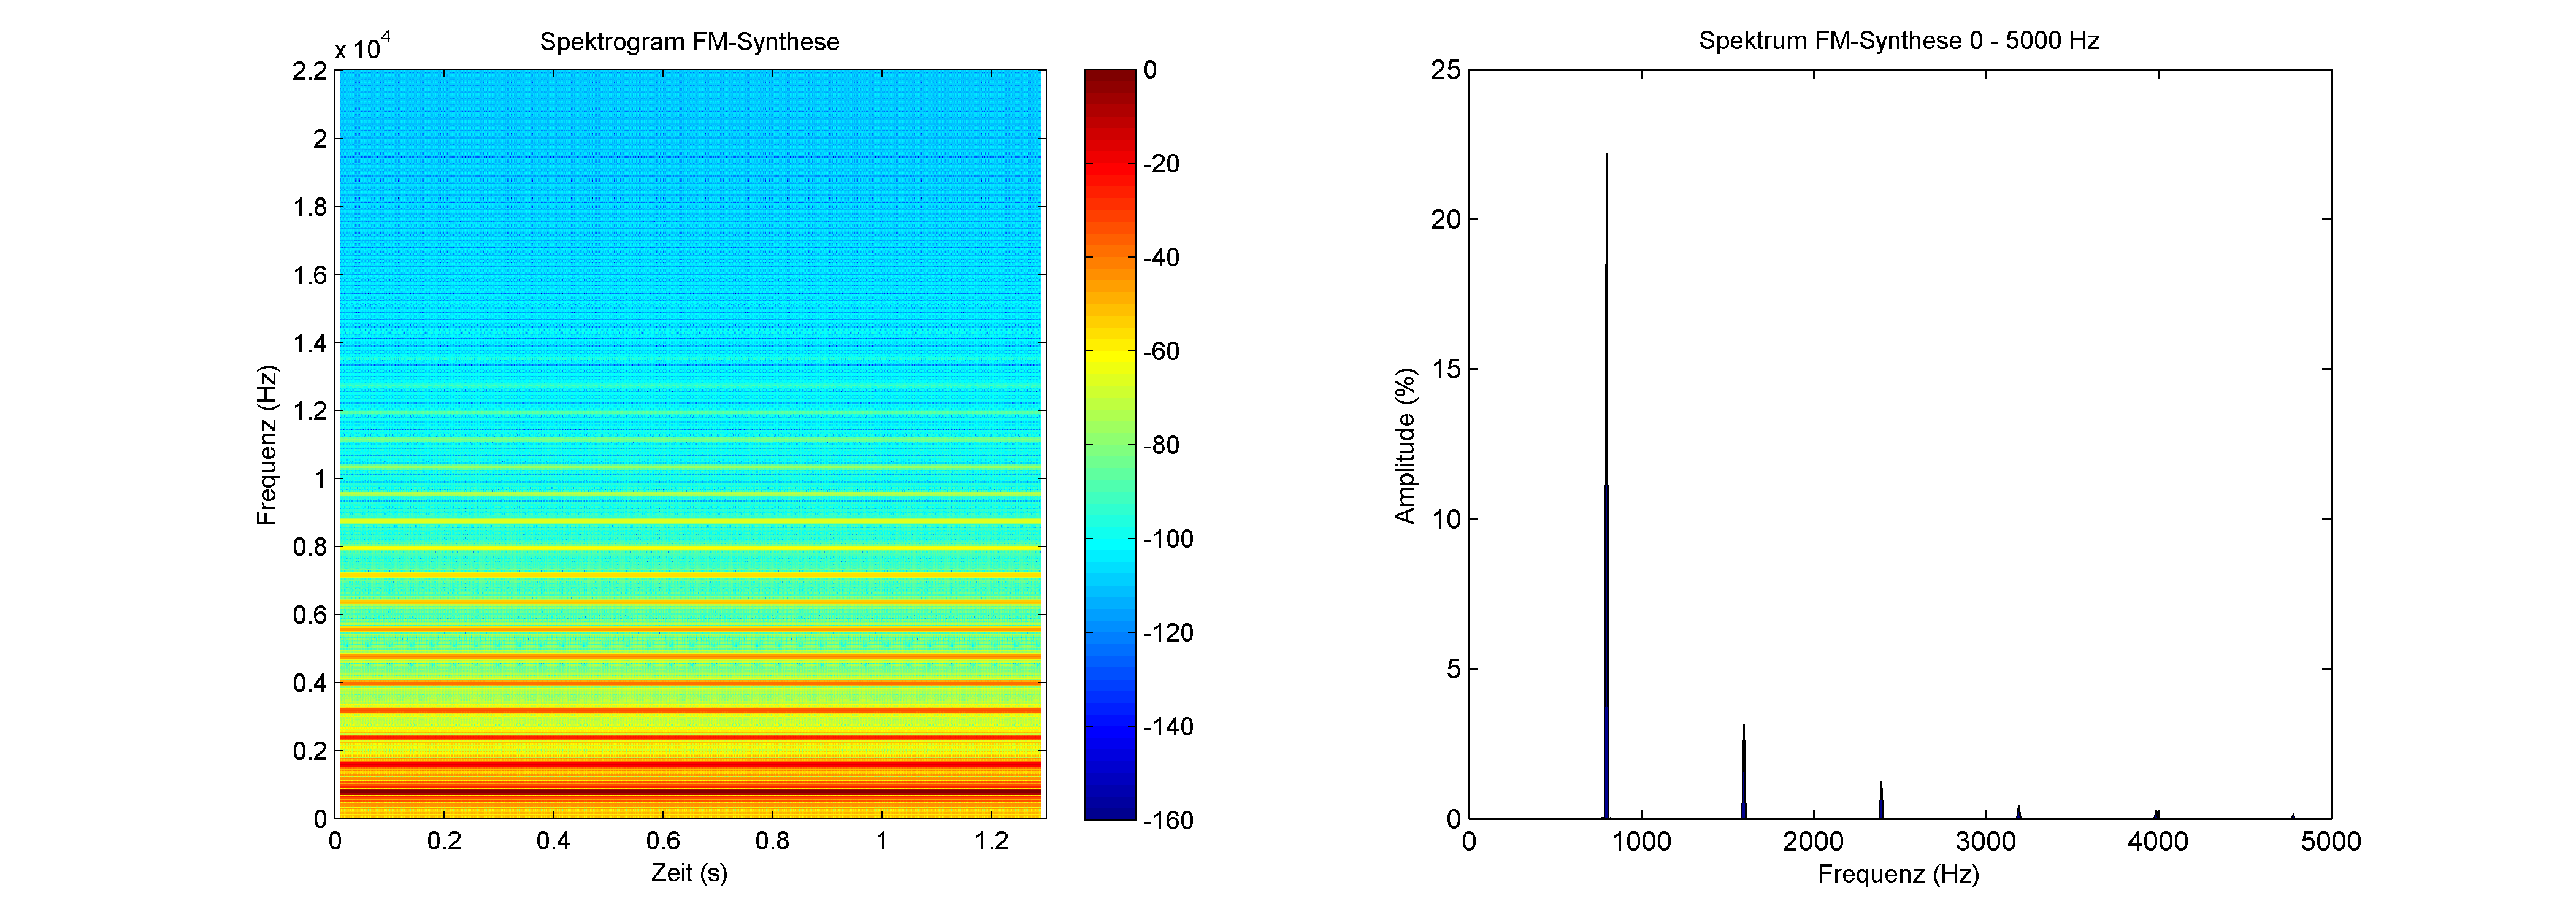
\includegraphics[width=1\textwidth]{plotFMSyntheseKomplex4Mod.png}
\caption{Plot des Spektrograms und des Spektrums der FM-Synthese mit 4 Modulatoren und den Parametern fc = 796.75 Hz, fm1 = fm2 = fm3 = fm4 = fc, I1 = 0.3, I2 = 0.5, I3 = 1 und I4 = 1}
\label{fig:plotFMSyntheseKomplex4Mod}
Quelle: Eigene Darstellung mit Matlab
\end{figure}

Da die Grundeinstellung der FM-Synthese mit den oben genannten Parametern ein zufriedenstellendes Signal erzeugt, können wir uns jetzt der Veredlung des Tones widmen. Durch Hinzufügen eines Vibratos wirkt der erzeugte Klang lebendiger und nicht ganz so künstlich. Dies kann bewerkstelligt werden indem die Modulationsfrequenz leicht erhöht oder verringert wird. Auch hierbei muss experimentiert werden, welche Erhöhung der Modulationsfrequenz das gewünschte Ergebnis erzeugt. Als sehr ähnlich zum Original Ton hat sich in diesem Fall eine Erhöhung um 2.5 Hz herausgestellt. Unsere neue Modulationsfrequenz ist somit fm = fc + 2.5. In Abbildung \ref{fig:spektrumFMSyntheseVibrato} wird die Auswirkung des Vibratos sichtbar, es bilden sich um die Seitenfrequenzen weitere recht gering ausgeprägte Frequenzausschläge. Der Vibrato führt zu einer leichten Schwingung des Tones. 

\begin{figure} [ht]
\centering
  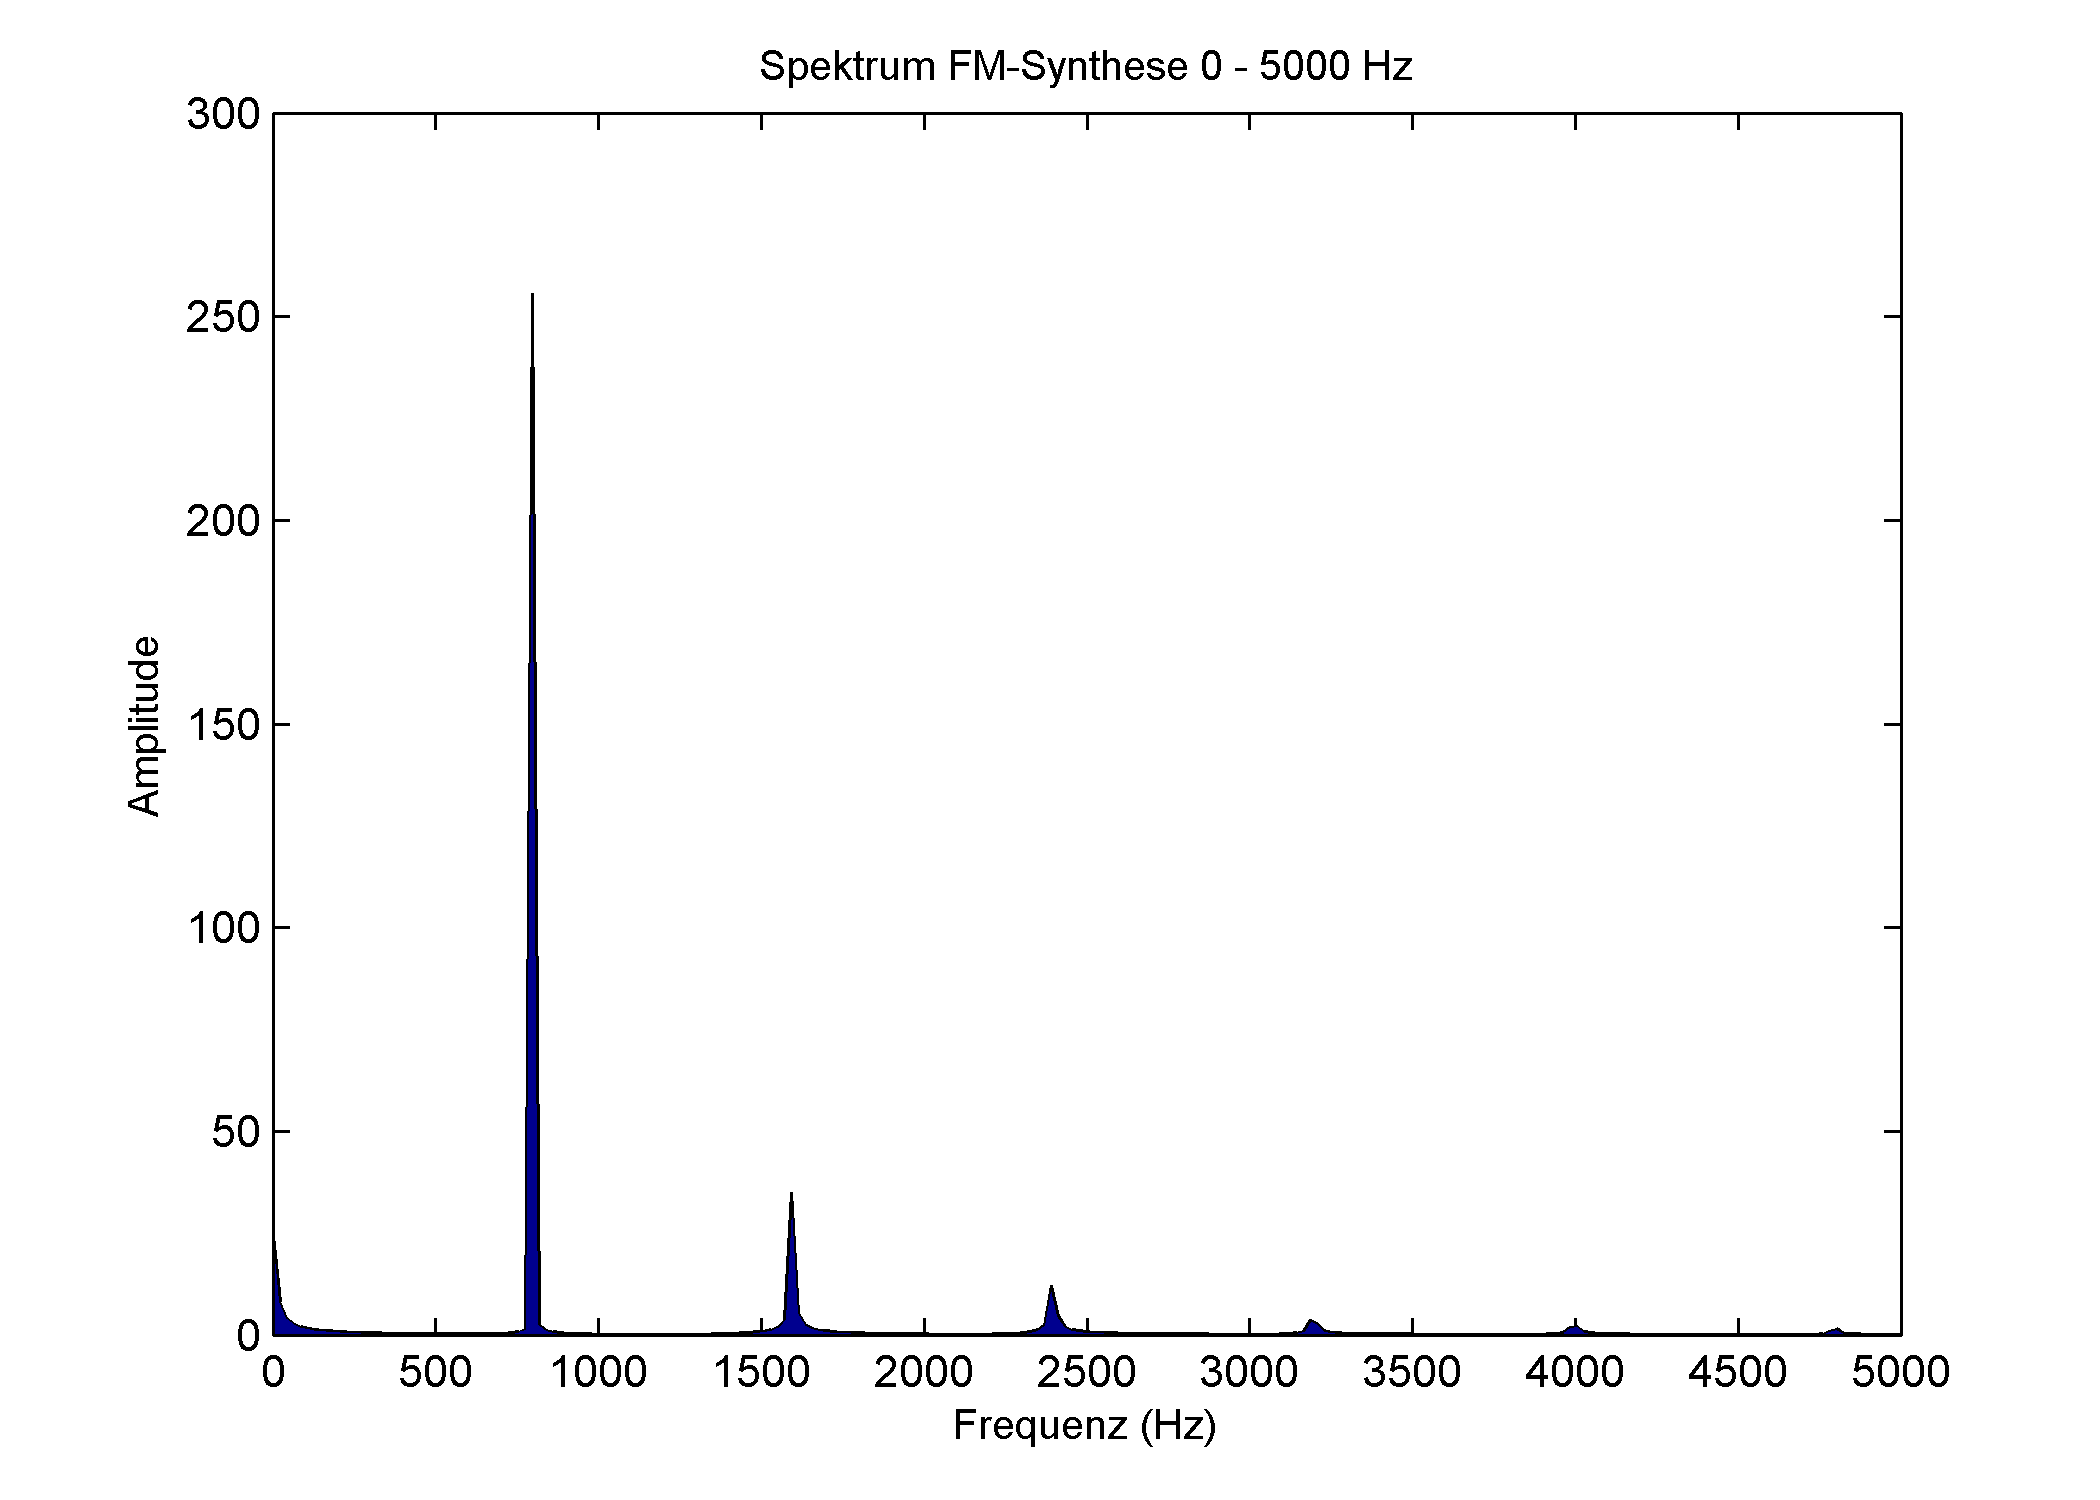
\includegraphics[width=0.5\textwidth]{spektrumFMSyntheseVibrato.png}
\caption{Plot des Spektrums der FM-Synthese mit 4 Modulatoren und Vibrato fm1 = fm2 = fm3 = fm4 = fc + 2.5}
\label{fig:spektrumFMSyntheseVibrato}
Quelle: Eigene Darstellung mit Matlab
\end{figure}

Der nächste wichtige und einfach hinzuzufügende Bestandteil des synthetisierten Tones ist die ADSR-Hüllkurve. Um generell eine Querflöte nachzumachen wäre eine Hüllkurve wie in Abbildung \ref{fig:adsrFluteGeneral} gezeigt möglich. Allerdings versuchen wir den originalen Ton der Querflöte so gut wie möglich nachzuahmen, hierfür wurde eine Komplexere Hüllkurve nach dem Beispiel der Waveform des original Tones generiert. Bei dieser Hüllkurve wurde Attack, Decay und Release von der Allgemeinen Hüllkurve übernommen und die Sustain Phase angepasst, zu sehen in Abbildung \ref{fig:adsrFluteComplex}. 

\begin{figure} [ht]
\centering
  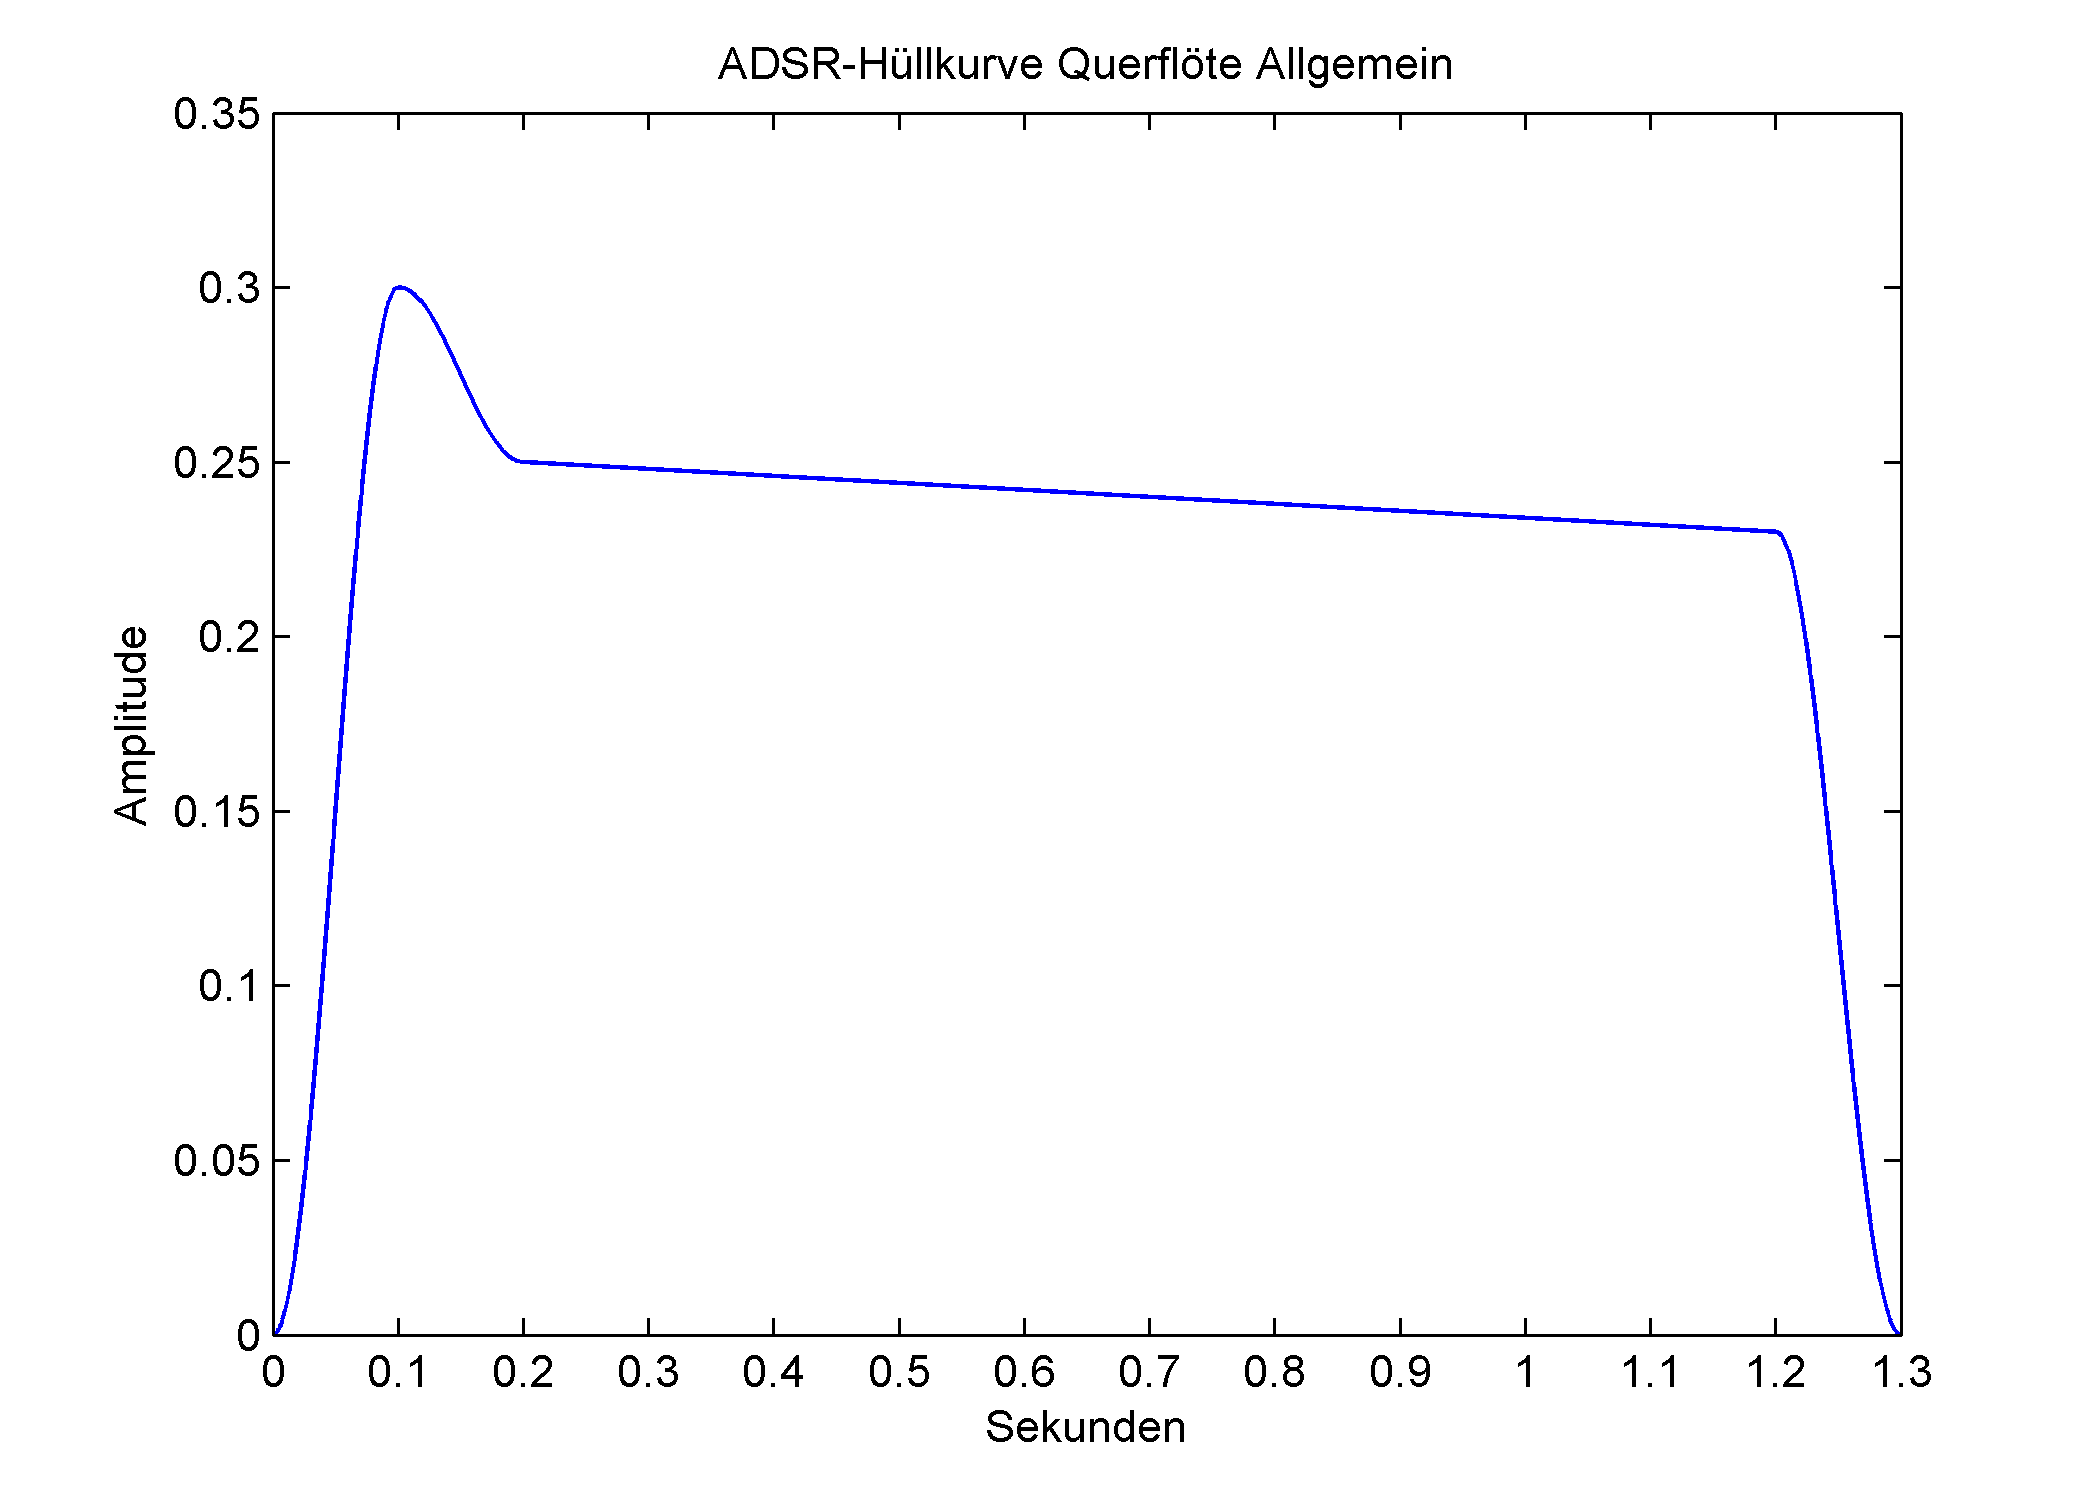
\includegraphics[width=0.5\textwidth]{adsrFluteGeneral.png}
\caption{Plot der ADSR-Hüllkurve einer Querflöte}
\label{fig:adsrFluteGeneral}
Quelle: Eigene Darstellung mit Matlab
\end{figure}

\begin{figure} [ht]
\centering
  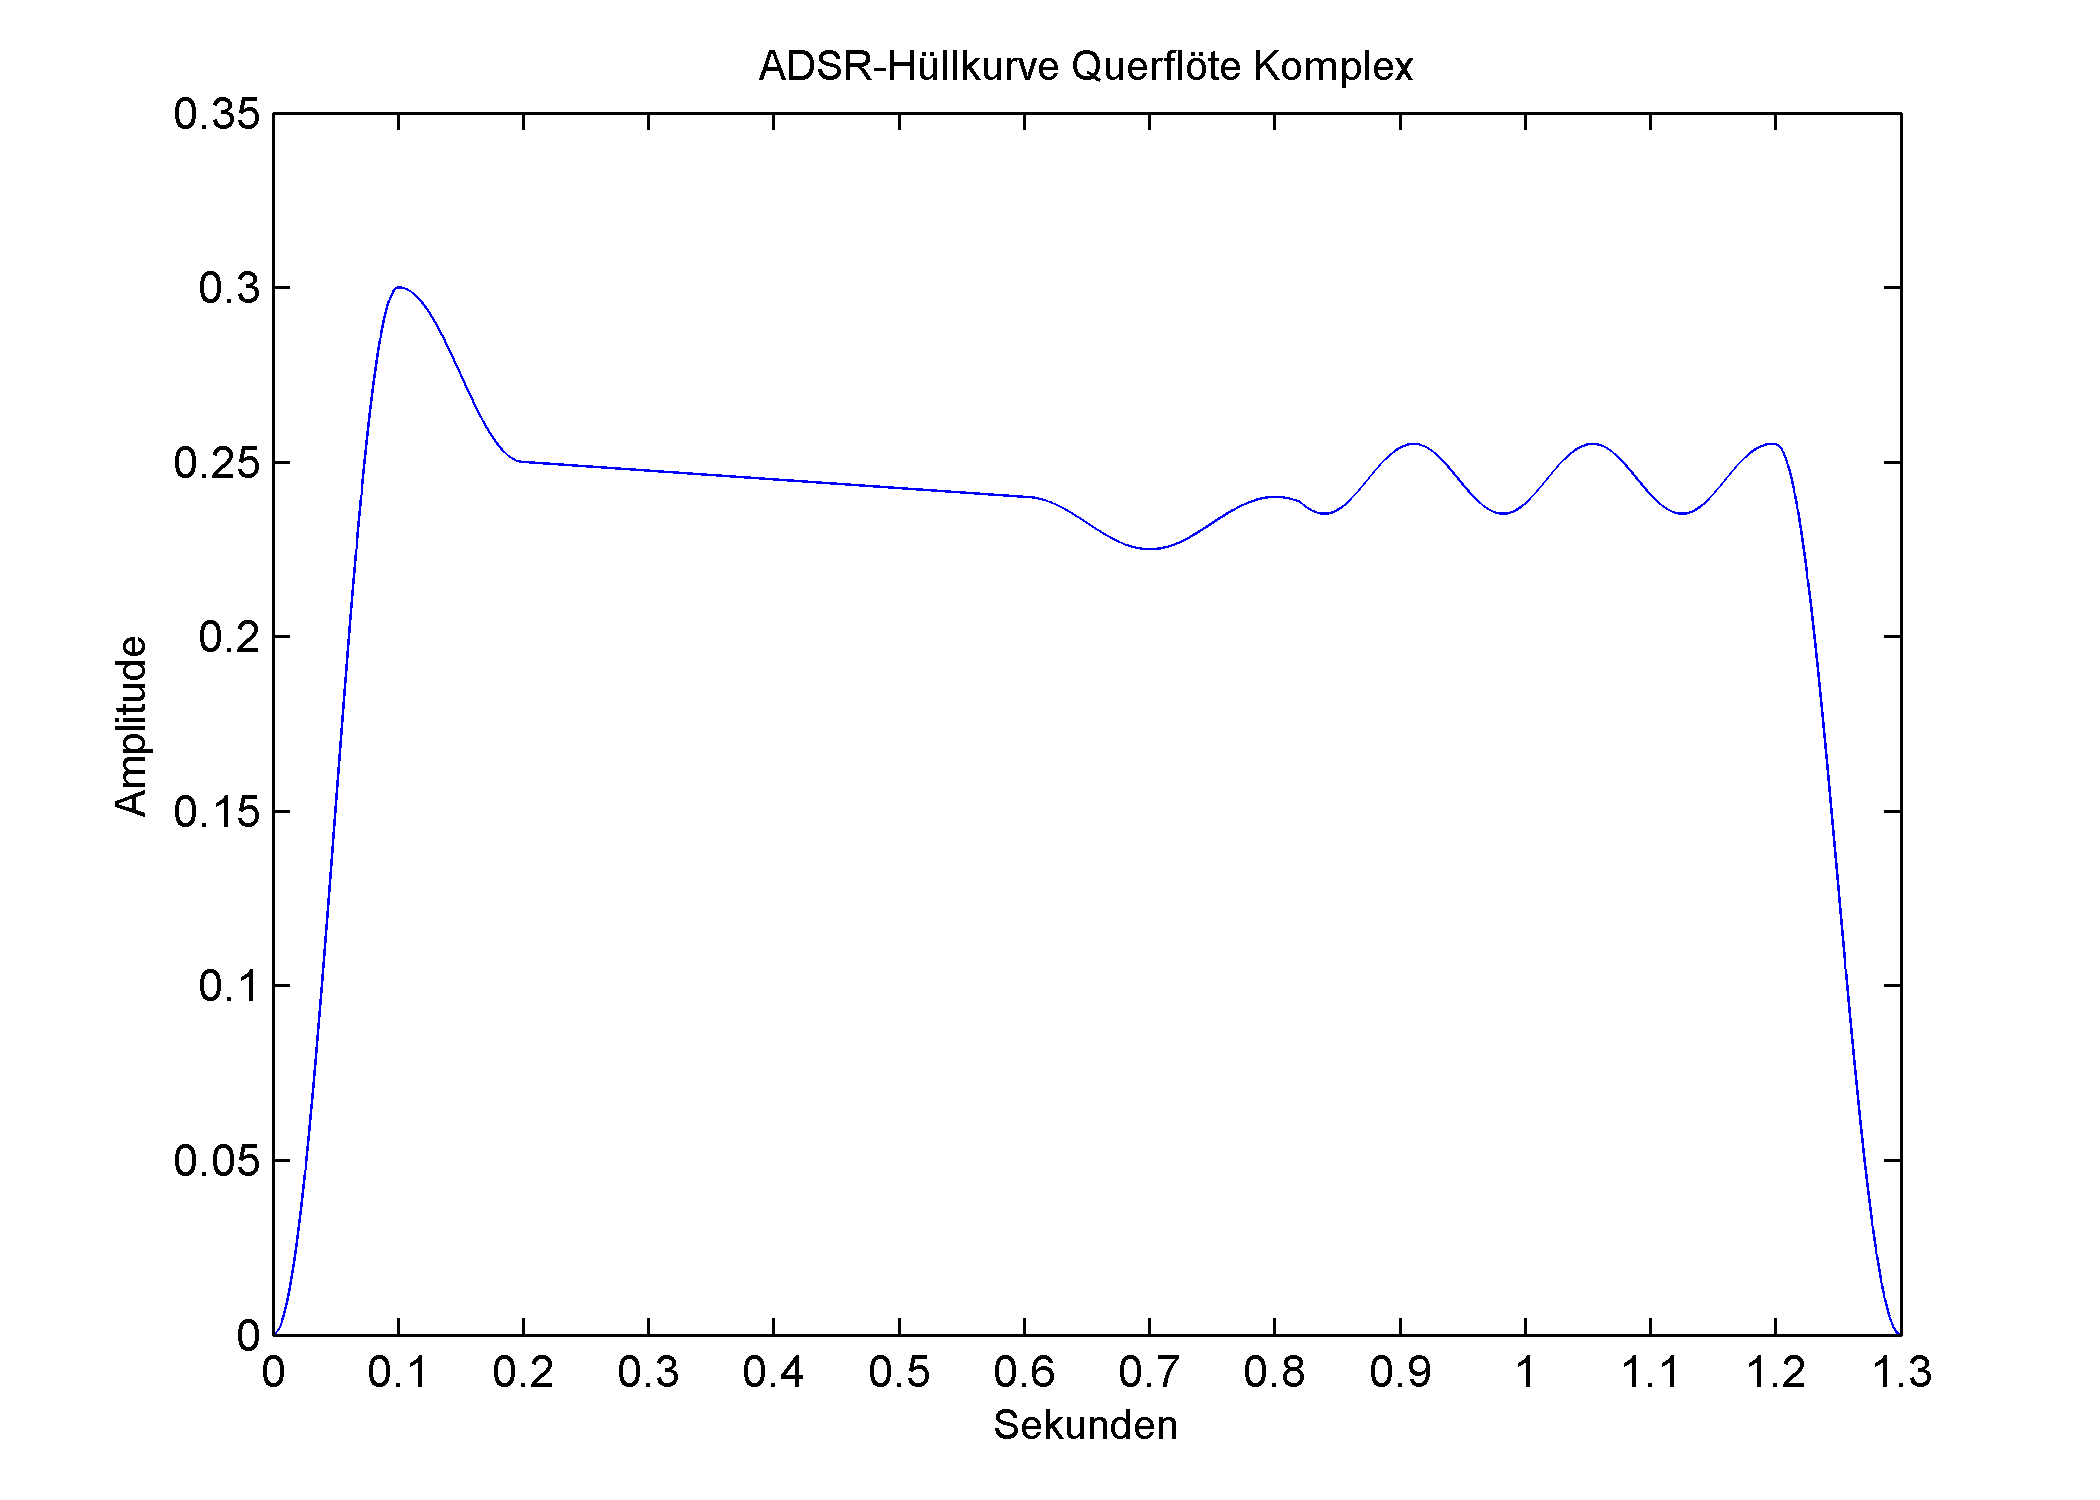
\includegraphics[width=0.5\textwidth]{adsrFluteComplex.png}
\caption{Plot der Komplexen ADSR-Hüllkurve dieses Querflötentones}
\label{fig:adsrFluteComplex}
Quelle: Eigene Darstellung mit Matlab
\end{figure}

Nachdem Vibrato und ADSR-Hüllkurve hinzugefügt wurden, hat sich das Spektrogram zur Abbildung \ref{fig:plotFMSyntheseKomplex4Mod} kaum geändert. Es wird nur der Vibrato durch die etwas breiteren Seitenfrequenzen und die ADSR-Hüllkurve durch ansteigen des Spektrums zu Beginn des Tones und Abfallen des Spektrums nach 1.2 Sekunden sichtbar. Der Ton hört sich von der Tonhöhe und der Intensität schon stark nach dem Original Querflöten Ton an. Allerdings fehlen noch die Typischen Blas- und Luftverwirblungsgeräusche sowie das sehr starke Anblasgeräusch.

\FloatBarrier

FM Parametrisierung mittels Genetischer Algorithmen

Mittels genetischer Algorithmen ist es möglich Parameter der FM Synthese herauszufinden, die nötig sind um einen Ton zu erzeugen der nach einem echten Instrument klingt. Diese Algorithmen zerlegen einen echten Ton eines Instrumentes mittels Schneller Fourier Transformation in seine einzelnen Bestandteile und versucht verschiedene Parameter für die Synthese aus, zerlegt das entstandene Signal wieder mittels Schneller Fourier Transformation und vergleicht die Ergebnisse. Mit diesem Verfahren können recht zuverlässig realistisch Synthetisierte Töne erzeugt werden, die von einem Originalen Instrument kaum zu unterscheiden sind. Da für die Implementierung eines solchen Algorithmus allerdings die Zeit fehlt, wird dieses Thema in dieser Arbeit nicht weiter vertieft. Eine Ausführliche Erklärung der FM Parametrisierung mittels Genetischer Algorithmen kann in Andrew Horners Artikel "Nested Modulator and Feedback FM Matching of Instrument Tones" nachgelesen werden.


Doppel Modulator FM
x(t) = w(t) sin[2*pi*fc*t + Im1*sin(2*pi*fm1*t) + Im2*sin(2*pi*fm2*t)];

Geschachtelte FM Modulation
x(t) = w(t)*sin{2*pi*fc*t + Im1*sin[2*pi*fm1*t + Im2*sin(2*pi*fm2*t)]}

Feedback FM 
xn = wn *sin[(2*pi*f1n/SR)+(B*xn-1/wn-1)]

\FloatBarrier
\subsubsection{Modulationsframework (Theorie -> Praxis)}
\FloatBarrier
\subsubsection{Demo: Parameter und Effekte - Grafiken (evtl. Plotten)}